\section{Cobordism 3}
Suppose we have 
\begin{itemize}
\item a punctured Riemann sphere $M$

\item co-oriented link $\Lambda_0 = (\Phi_0,\xi_0)$ about $0$

\item co-oriented link $\Lambda_\infty = (\Phi_\infty,\xi_\infty)$ about $\infty$ 

\item a co-oriented lines $\Lambda_{squig} = (\Phi_{squig}, \xi_{squig})$ that refines the stratification induced by $\Lambda_0 \coprod \Lambda_\infty$ to a regular cell complex 
\end{itemize}
and suppose we have a nested disk $D' \subset D \subset M$ and a smooth chart
\[
	f: \{(x,z)\in \R^2 ~|~ x^2+z^2 < 4 \} \rightarrow D
\]
such that 
\begin{itemize}
\item $\{(x,z)\in \R^2 ~|~ x^2+z^2 < 1\}$ is mapped to $D'$ 

\item I will abuse the notation so that $D'$ denotes $\{(x,z)\in \R^2 ~|~ x^2+z^2 < 1\}$ and $D$ denotes $\{(x,z)\in \R^2 ~|~ x^2+z^2 < 4 \}$

\item $\{(x,z)\in D' ~|~ z = -\frac{5}{3}x^2 + \frac{3}{4} \}$, co-oriented downward, is mapped to $\Lambda_0 |_{D'}$

\item $\{(x,z)\in D' ~|~ z = \frac{1}{2} \}$, co-oriented upward, is mapped to $\Lambda_\infty |_{D'}$

\item $\{(x,z)\in D' ~|~ x = 0 \}$, co-oriented leftward, is mapped to $\Lambda_{squig} |_{D'}$
\end{itemize}
Suppose we have a sheaf $\mathfrak{F}$ singular supported on $\Lambda_0 \coprod \Lambda_\infty \coprod \Lambda_{squig}$, $f^*\mathfrak{F}$ is described as the following legible diagram.

\begin{definition}
\[
s_0(sgn_1,sgn_2,sgn_3):=~ \{(x,z) \in D' ~|~ sgn(z+\frac{5}{3}x^2 - \frac{3}{4})=sgn_1,~ sgn(-\frac{1}{2}-z)=sgn_2,~ sgn(x)=sgn_3 \}
\]
\end{definition}

Note that $\Lambda_0 \coprod \Lambda_\infty \coprod \Lambda_{squig}$ divides $D'$ into $8$ regions which are
\[
	\{s_0(+,-,-) ~|~ sgn_1, sgn_2, sgn_3 \in \{-,+\} \}
\]

The legible diagram for $f^*\mathfrak{F}$ is given as follows\\
\textbf{Stalks:}
\begin{itemize}
\item $F_0(s_0(-,-,sgn_3))$ := $\mathbb{C}^{m}$
\item $F_0(s_0(+,-,sgn_3))$ := $\mathbb{C}^{m+1}$
\item $F_0(s_0(-,+,sgn_3))$ := $\mathbb{C}^{m+1}$
\item $F_0(s_0(+,+,sgn_3))$ := $\mathbb{C}^{m+2}$
\end{itemize}
where $sgn_3 \in \{-, + \}$.\\
\textbf{Generization maps:}
\begin{itemize}
\item $F_0(s_0(0,sgn_2,sgn_3)):~ F_0(s_0(-,sgn_2,sgn_3))\rightarrow F_0(s_0(+,sgn_2,sgn_3))$ := $\iota_1$ 

\item $F_0(s_0(sgn_1,0,sgn_3)):~ F_0(s_0(sgn_1,-,sgn_3))\rightarrow F_0(s_0(sgn_1,+,sgn_3))$ := $\iota_0$ 

\item $F_0(s_0(-,-,0)):~ F_0(s_0(-,-,-))\rightarrow F_0(s_0(-,-,+))$ := $T(2,2,m+1,m+1)$ 

\item $F_0(s_0(+,-,0)):~ F_0(s_0(+,-,-))\rightarrow F_0(s_0(+,-,+))$ := $T(2,2,m+2,m+2)$ 

\item $F_0(s_0(-,+,0)):~ F_0(s_0(-,+,-))\rightarrow F_0(s_0(-,+,+))$ := $T(1,1,m+1,m+1)$ 

\item $F_0(s_0(+,+,0)):~ F_0(s_0(+,+,-))\rightarrow F_0(s_0(+,+,+))$ := $T$ 
\end{itemize}
Here, $T$ is a matrix that gives rise to a linear transformation from $\C^{m+2}$ to $\C^{m+2}$ where
\begin{itemize}
\item $T(span\{ e_2, \cdots, e_{m+1} \}) \subset span\{ e_2, \cdots, e_{m+1} \}$

\item $T(span\{ e_1, \cdots, e_{m+1} \}) \subset span\{ e_1, \cdots, e_{m+1} \}$

\item $T(span\{ e_2, \cdots, e_{m+2} \}) \subset span\{ e_2, \cdots, e_{m+2} \}$
\end{itemize}
and $T(r_{start},r_{end},c_{start},c_{end})$ is the submatrix of $T$ that contains rows from $r_{start}$ to $r_{end}$ and columns from $c_{start}$ to $c_{end}$.\\

Now I will define a cobordism of $f^*\mathfrak{F}$, say $Cobordism_3$ that satisfies the following conditions
\begin{itemize}
\item $Cobordism_3$ is supported on $overline{D}$

\item $Cobordism_3$ inside of $D-D'$ is perturbed so that $\Lambda$'s remain smooth link throughout the isotopy but won't exactly describe what it is

\item I will only describe $Cobordism_3$ inside $D'$
\end{itemize}
Now let's define $Cobordism_3$ as a legible diagram on $D'\times [0,1]_t$ whose regions are the regions separated by the following hyperplanes corresponding to the world sheets of $\Lambda_0$, $\Lambda_\infty$, and $\Lambda_{squig}$
\begin{itemize}
\item world sheet of $\Lambda_0$: 
$\{(x,z,t) \in D' \times [0,1] ~|~ z=\frac{5}{3}(1-t)x^2 - \frac{5}{4}t+\frac{3}{4}\}$, where hairs are pointing downward. Note that when $t=t_0$, the above set is the parabola passing through $(-\frac{\sqrt{3}}{2}, -\frac{1}{2})$, $(\frac{\sqrt{3}}{2}, -\frac{1}{2})$, and $(0,-\frac{5}{4}t_0 + \frac{3}{4})$.

\item world sheet of $\Lambda_\infty$: 
$\{(x,z,t) \in D' \times [0,1] ~|~ z=\frac{1}{2} \}$, where hairs are pointing upward.

\item world sheet of $\Lambda_{squig}$:
$\{(x,z,t) \in D' \times [0,1] ~|~ x=0 \}$, where hairs are pointing leftward.
\end{itemize}
\begin{definition}
\begin{align*}
s(sgn_1,sgn_2,sgn_3) :=~ &\{(x,z,t) \in D' \times [0,1] ~|~ sgn(z+\frac{5}{3}(1-t)x^2+\frac{5}{4}t-\frac{3}{4}) = sgn_1, \\
& sgn(-\frac{1}{2}-z)=sgn_2,sgn(x)=sgn_3
	\}
\end{align*}
\end{definition}
The above three world sheets separate $D'\times [0,1]$ into $8$ regions
\[
	\{s(sgn_1,sgn_2,sgn_3) ~|~ sgn_1,sgn_2,sgn_3 \in \{-,+\}\}
\]
and we get the following stratification
\[
	\mathcal{S} = \{ s(sgn_1,sgn_2,sgn_3) ~|~ sgn_1,sgn_2, sgn_3 \in \{-,0,+\} \}
\]
Now let's define a legible diagram $F$ as follows
\textbf{Stalks:}
\begin{itemize}
\item $F_0(s_0(-,-,sgn_3))$ := $\mathbb{C}^{m}$
\item $F_0(s_0(+,-,sgn_3))$ := $\mathbb{C}^{m+1}$
\item $F_0(s_0(-,+,sgn_3))$ := $\mathbb{C}^{m+1}$
\item $F_0(s_0(+,+,sgn_3))$ := $\mathbb{C}^{m+2}$
\end{itemize}
where $sgn_3 \in \{-, + \}$.\\
\textbf{Generization maps:}
\begin{itemize}
\item $F_0(s_0(0,sgn_2,sgn_3)):~ F_0(s_0(-,sgn_2,sgn_3))\rightarrow F_0(s_0(+,sgn_2,sgn_3))$ := $\iota_1$ 

\item $F_0(s_0(sgn_1,0,sgn_3)):~ F_0(s_0(sgn_1,-,sgn_3))\rightarrow F_0(s_0(sgn_1,+,sgn_3))$ := $\iota_0$ 

\item $F_0(s_0(-,-,0)):~ F_0(s_0(-,-,-))\rightarrow F_0(s_0(-,-,+))$ := $T(2,2,m+1,m+1)$ 

\item $F_0(s_0(+,-,0)):~ F_0(s_0(+,-,-))\rightarrow F_0(s_0(+,-,+))$ := $T(2,2,m+2,m+2)$ 

\item $F_0(s_0(-,+,0)):~ F_0(s_0(-,+,-))\rightarrow F_0(s_0(-,+,+))$ := $T(1,1,m+1,m+1)$ 

\item $F_0(s_0(+,+,0)):~ F_0(s_0(+,+,-))\rightarrow F_0(s_0(+,+,+))$ := $T$ 
\end{itemize}
Here, $T$ is a matrix that gives rise to a linear transformation from $\C^{m+2}$ to $\C^{m+2}$ where
\begin{itemize}
\item $T(span\{ e_2, \cdots, e_{m+1} \}) \subset span\{ e_2, \cdots, e_{m+1} \}$

\item $T(span\{ e_1, \cdots, e_{m+1} \}) \subset span\{ e_1, \cdots, e_{m+1} \}$

\item $T(span\{ e_2, \cdots, e_{m+2} \}) \subset span\{ e_2, \cdots, e_{m+2} \}$
\end{itemize}
and $T(r_{start},r_{end},c_{start},c_{end})$ is the submatrix of $T$ that contains rows from $r_{start}$ to $r_{end}$ and columns from $c_{start}$ to $c_{end}$.
\begin{proposition}
The above diagram is a well-defined legible diagram.
\end{proposition}
\begin{proof}
It is enough to show that the total complexes of the subdiagrams the above defined diagram associated to sub-penultimate dimensional strata.
\end{proof}
\begin{figure}[H] 
    \centering
    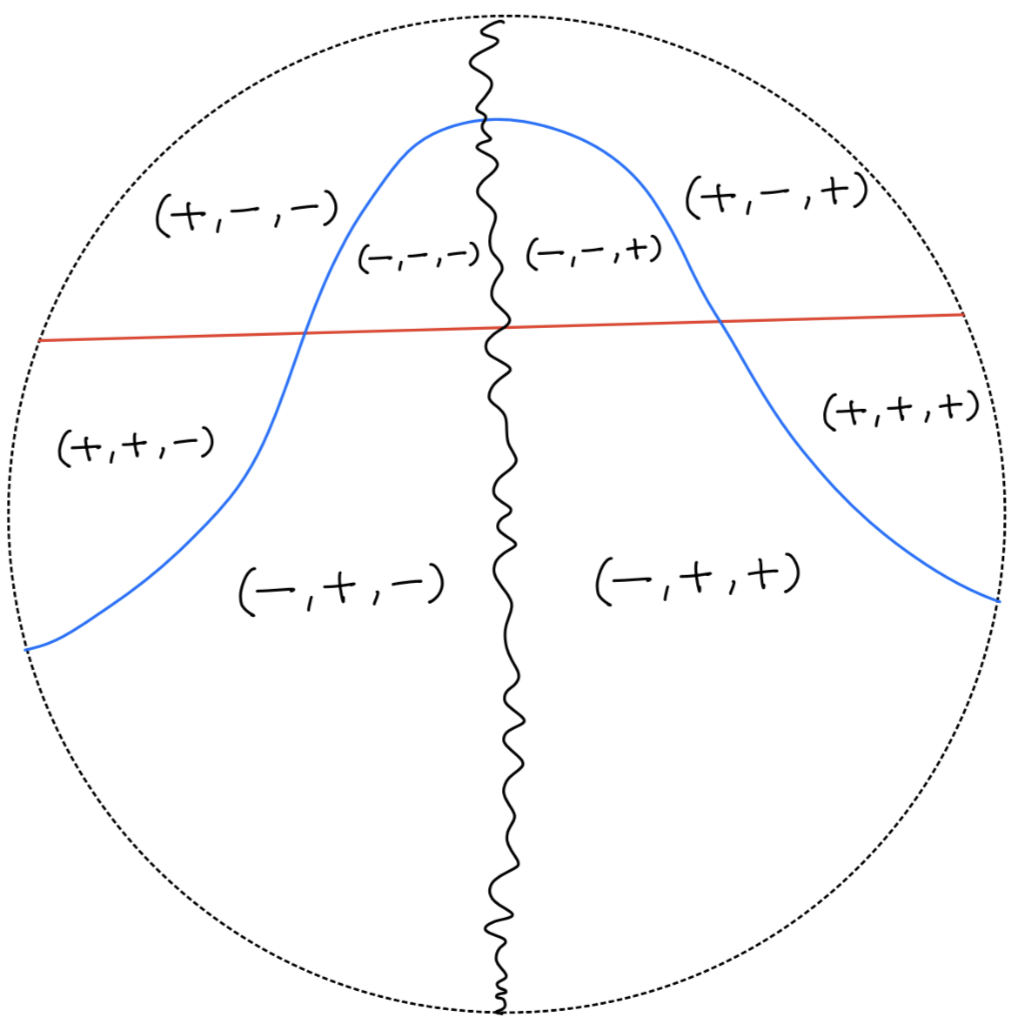
\includegraphics[scale = 0.95]{diagrams/lemma3/1.png} 
    \caption{Your caption here}
    \label{fig:your-label}
\end{figure}


\begin{figure}[H] 
    \centering
    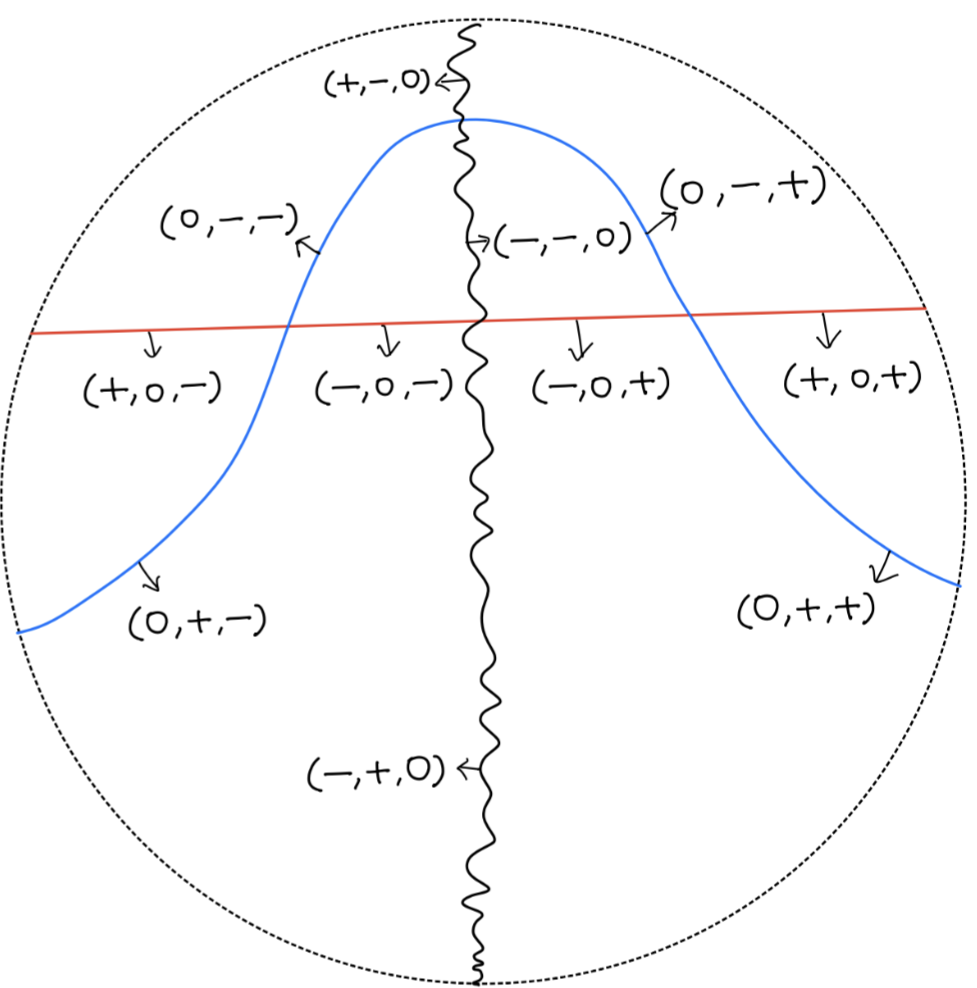
\includegraphics[scale = 0.95]{diagrams/lemma3/2.png} 
    \caption{Your caption here}
    \label{fig:your-label}
\end{figure}